\batchmode
\makeatletter
\def\input@path{{\string"C:/Users/Hao/Dropbox/NewtermPHD/TERM2/SS9833B Analysis of brain imaging data/Report/\string"/}}
\makeatother
\documentclass[english]{article}\usepackage[]{graphicx}\usepackage[]{color}
%% maxwidth is the original width if it is less than linewidth
%% otherwise use linewidth (to make sure the graphics do not exceed the margin)
\makeatletter
\def\maxwidth{ %
  \ifdim\Gin@nat@width>\linewidth
    \linewidth
  \else
    \Gin@nat@width
  \fi
}
\makeatother

\definecolor{fgcolor}{rgb}{0.345, 0.345, 0.345}
\newcommand{\hlnum}[1]{\textcolor[rgb]{0.686,0.059,0.569}{#1}}%
\newcommand{\hlstr}[1]{\textcolor[rgb]{0.192,0.494,0.8}{#1}}%
\newcommand{\hlcom}[1]{\textcolor[rgb]{0.678,0.584,0.686}{\textit{#1}}}%
\newcommand{\hlopt}[1]{\textcolor[rgb]{0,0,0}{#1}}%
\newcommand{\hlstd}[1]{\textcolor[rgb]{0.345,0.345,0.345}{#1}}%
\newcommand{\hlkwa}[1]{\textcolor[rgb]{0.161,0.373,0.58}{\textbf{#1}}}%
\newcommand{\hlkwb}[1]{\textcolor[rgb]{0.69,0.353,0.396}{#1}}%
\newcommand{\hlkwc}[1]{\textcolor[rgb]{0.333,0.667,0.333}{#1}}%
\newcommand{\hlkwd}[1]{\textcolor[rgb]{0.737,0.353,0.396}{\textbf{#1}}}%

\usepackage{framed}
\makeatletter
\newenvironment{kframe}{%
 \def\at@end@of@kframe{}%
 \ifinner\ifhmode%
  \def\at@end@of@kframe{\end{minipage}}%
  \begin{minipage}{\columnwidth}%
 \fi\fi%
 \def\FrameCommand##1{\hskip\@totalleftmargin \hskip-\fboxsep
 \colorbox{shadecolor}{##1}\hskip-\fboxsep
     % There is no \\@totalrightmargin, so:
     \hskip-\linewidth \hskip-\@totalleftmargin \hskip\columnwidth}%
 \MakeFramed {\advance\hsize-\width
   \@totalleftmargin\z@ \linewidth\hsize
   \@setminipage}}%
 {\par\unskip\endMakeFramed%
 \at@end@of@kframe}
\makeatother

\definecolor{shadecolor}{rgb}{.97, .97, .97}
\definecolor{messagecolor}{rgb}{0, 0, 0}
\definecolor{warningcolor}{rgb}{1, 0, 1}
\definecolor{errorcolor}{rgb}{1, 0, 0}
\newenvironment{knitrout}{}{} % an empty environment to be redefined in TeX

\usepackage{alltt}
\usepackage{ae,aecompl}
\usepackage[T1]{fontenc}
\usepackage[latin9]{inputenc}
\usepackage{geometry}
\geometry{verbose,tmargin=1.1cm,bmargin=2.2cm,lmargin=2cm,rmargin=2cm}
\setcounter{tocdepth}{-1}
\usepackage{color}
\usepackage{babel}
\usepackage{float}
\usepackage{url}
\usepackage{amsmath}
\usepackage{fixltx2e}
\usepackage{graphicx}
\usepackage[unicode=true,pdfusetitle,
 bookmarks=false,
 breaklinks=true,pdfborder={0 0 1},backref=false,colorlinks=true]
 {hyperref}

\makeatletter
%%%%%%%%%%%%%%%%%%%%%%%%%%%%%% Textclass specific LaTeX commands.
\usepackage{enumitem}		% customizable list environments
\newlength{\lyxlabelwidth}      % auxiliary length 

\@ifundefined{showcaptionsetup}{}{%
 \PassOptionsToPackage{caption=false}{subfig}}
\usepackage{subfig}
\makeatother
\IfFileExists{upquote.sty}{\usepackage{upquote}}{}
\begin{document}

\title{Introduction to MANOVA and CV-MANOVA}


\author{Yuanhao Lai%
\thanks{\protect\url{ylai72@uwo.ca}, Department of Statistical and Actuarial
Sciences, Western University%
}}

\maketitle
\vspace{-30bp}



\section{MANOVA and CVMANOVA}


\subsection{Model Structure}

The method, multivariate analysis of variance (MANOVA)\cite{fox2013hypothesis},
assumes our data are generated from the multivariate general linear
model (MGLM), 
\[
\underset{\left(n\times p\right)}{\boldsymbol{Y}}=\underset{\left(n\times k\right)}{\boldsymbol{Z}}\underset{\left(k\times p\right)}{\boldsymbol{U}}+\underset{\left(n\times p\right)}{\boldsymbol{E}}
\]
where $\boldsymbol{Y}$ specifies the signal at $n$ different time
points in $p$ voxels, $\boldsymbol{Z}$ is the design matrix with
$K$ conditions such as the constant, linear predictors, dummy variables
for categorical predictors, $\boldsymbol{U}$ is a matrix of regression
coefficients and $\boldsymbol{E}$ is a matrix of random errors. It
is assumed that $Z$ is of full column-rank $k$ and each of the $n$
rows of $E$ is an independent sample from a $p$-dimensional normal
distribution $\text{N}(\boldsymbol{0},\Sigma_{\epsilon})$. $\Sigma_{\epsilon}$
is the spatial covariance structure of the data. Notice that $n=m\times k$,
where $m$ is the number of runs.

The maximum likelihood estimator (MLE) for $\boldsymbol{U}$ is, 
\[
\hat{\boldsymbol{U}}=\left(\boldsymbol{Z}^{T}\boldsymbol{Z}\right)^{-1}\boldsymbol{Z}^{T}\boldsymbol{Y}
\]



\subsection{Hypothesis Test}

We are interested in testing if there is any difference between patterns.
The null hypothesis is set as, 
\[
H_{0}:\ \underset{\left(q\times k\right)}{\boldsymbol{C}^{T}}\underset{\left(k\times p\right)}{\boldsymbol{U}}=\boldsymbol{0}
\]
where $\boldsymbol{C}$ is a $k\times q$ a contrast matrix of the
parameters, with rank $q\le k$.


\subsection{MANOVA\label{sub:MANOVA}}

To construct a test statistic, we first define the following two important
components, which are similar to the uni-variate case.

The regression sum of square, 
\begin{equation}
\boldsymbol{Q}_{h}=\hat{\boldsymbol{U}}^{T}\boldsymbol{H}^{T}\boldsymbol{Z}^{T}\boldsymbol{Z}\boldsymbol{H}\hat{\boldsymbol{U}}\label{eq:MANOVAQh}
\end{equation}
where $\boldsymbol{H}=\boldsymbol{C}\left(\boldsymbol{C}^{T}\boldsymbol{C}\right)^{-1}\boldsymbol{C}^{T}$
is the hypothesis matrix corresponding to the contrast $\boldsymbol{C}$.

The residual sum of square,
\begin{equation}
\boldsymbol{Q}_{e}=\left(\boldsymbol{Y}-\boldsymbol{Z}\hat{\boldsymbol{U}}\right)^{T}\left(\boldsymbol{Y}-\boldsymbol{Z}\hat{\boldsymbol{U}}\right)\label{eq:MANOVAQe}
\end{equation}
which is also an estimator for the (spatial) covariance structure
$\Sigma_{\epsilon}$ of the data, as $\hat{\Sigma}_{\epsilon}=\frac{1}{n}\boldsymbol{Q}_{e}$.

Using $\boldsymbol{Q}_{h}$ and $\boldsymbol{Q}_{e}$, we can construct
three types of test statistics for MANOVA, namely, the Wilks' lambda,
the Pillai's trace and the Barlett-Lawley-Hottellings trace. Those
statistics are different in the power in different situations. Normally,
Wilks' lambda is used as it is a likelihood ratio test statistic and
it is ensured to be the uniformly most powerful test though not the
most powerful test in a certain case. Wilks' lambda is defined as
below,

\begin{equation}
\Lambda=\frac{\det\left(\boldsymbol{Q}_{e}\right)}{\det\left(\boldsymbol{Q}_{h}+\boldsymbol{Q}_{e}\right)}=\prod_{i}\frac{1}{1+\lambda_{i}}
\end{equation}
where $\lambda_{i}$ are the solutions of the characteristic equation
$\mid\boldsymbol{Q}_{h}-\lambda\boldsymbol{Q}_{e}\mid=0$.

In addition, the $F$ approximation \cite{rao1951asymptotic} to the
null distribution of Wilks's Lambda is available, 
\[
F=\left[\Lambda^{\frac{-1}{t_{3}}}-1\right]\cdot\frac{\text{df}_{2}}{\text{df}_{1}}\sim F_{\text{df}_{1},\text{df}_{2}}
\]
where $t_{1}=n-k-\frac{p-q+1}{2}$, $t_{2}=\frac{pq-2}{4}$, $t_{3}=\begin{cases}
\sqrt{\frac{\left(pq\right)^{2}-4}{p^{2}+q^{2}-5}}, & p^{2}+q^{2}-5>0\\
1, & p^{2}+q^{2}-5\le0
\end{cases}$, $\text{df}_{1}=pq$ and $\text{df}_{2}=t_{1}\cdot t_{3}-2t_{2}$. 

\textbf{Notice} that the approximated $F$ distribution fails when
$n-k\ge p$ because $\text{df}_{2}$ may be less than $0$. The essential
reason is that $\boldsymbol{Q}_{e}$ defined by eqn.(\ref{eq:MANOVAQe})
is not positive-definite in this case and hence the computation of
the statistic is not feasible. To overcome this problem, we proposed
using the principle component analysis to reduce the number of voxels.
We would discuss it later in the Result section. 


\subsection{CV-MANOVA}

In the case where we want to quantify the distinctness between patterns,
we prefer the Barlett-Lawley-Hottellings trace because its equivalent
relationship to the Mahalanobis distance as shown by Allefeld \cite{allefeld2014searchlight}.
However, the Barlett-Lawley-Hottellings trace is severely biased,
so Allefeld used the cross-validated version of the Barlett-Lawley-Hottellings
trace to make it unbiased. The idea is very simple. He replaced the
estimated pattern $\hat{U}$ in eqn.(\ref{eq:MANOVAQh}) with its
cross-validated version. This alternative approach under the same
MGLM framework is called the cross-validated MANOVA (CV-MANOVA). The
resulted statistic by the \textquoteleft leave-one-run-out\textquoteright{}
cross-validation is,

\begin{equation}
D=\frac{(m-1)\left(n-k\right)-p-1}{(m-1)n}\cdot\frac{1}{m}\sum_{l=1}^{m}\sum_{h\neq l}\text{trace}\left[\boldsymbol{Q}_{h}^{CV}\left(\boldsymbol{Q}_{e}\right)^{-1}\right]\label{eq:CVMANOVA}
\end{equation}
where $\boldsymbol{Q}_{h}^{CV}=\hat{\boldsymbol{U}}^{(h)T}\boldsymbol{H}^{T}\boldsymbol{Z}^{(l)T}\boldsymbol{Z}^{(l)}\boldsymbol{H}\hat{\boldsymbol{U}}^{(l)}$
and $\hat{\boldsymbol{U}}^{(h)}$ is the MLE of $\boldsymbol{\boldsymbol{U}}$
using only the $h$th run data. However, CV-MANOVA suffered the same
problem as MANOVA for $\boldsymbol{Q}_{e}$ when $n-k\ge p$. But
since our simulated data is assumed to be (spatially) prewhitened
, $\boldsymbol{Q}_{e}=\hat{\Sigma}_{\epsilon}$ can be estimated as
a diagonal matrix where the diagonal elements are the same as eqn.(\ref{eq:MANOVAQe}).
However, there is not an exact distribution or a good approximated
distribution for this statistic. So the distribution under $H_{0}$
of the CV-MANOVA is obtained by either simulations or permutations. 


\section{Relationship between CV-MANOVA and RSA}

It can be shown the CV-MANOVA $D$ is also a linear contrasts of the
second moment matrix $\hat{G}$. If we ignored a constant scale of
the cross-validated Barlett-Lawley-Hottellings trace in eqn.(\ref{eq:CVMANOVA}),
then

\begin{eqnarray*}
D & = & \sum_{l=1}^{m}\sum_{h\neq l}\text{trace}\left[\boldsymbol{Q}_{h}^{CV}\left(\boldsymbol{Q}_{e}\right)^{-1}\right]\\
 & = & \sum_{l=1}^{m}\sum_{h\neq l}\text{trace}\left[\hat{\boldsymbol{U}}^{(h)T}\boldsymbol{H}^{T}\boldsymbol{Z}^{(l)T}\boldsymbol{Z}^{(l)}\boldsymbol{H}\hat{\boldsymbol{U}}^{(l)}\left(\hat{\Sigma}_{\epsilon}\right)^{-1}\right]\\
 & = & \sum_{l=1}^{m}\sum_{h\neq l}\text{trace}\left[\hat{\boldsymbol{U}}^{(h)T}\boldsymbol{H}^{T}\boldsymbol{Z}^{(l)T}\boldsymbol{Z}^{(l)}\boldsymbol{H}\hat{\boldsymbol{U}}^{(l)}\left(\hat{\Sigma}_{\epsilon}\right)^{-1}\hat{\boldsymbol{U}}^{(h)T}\right],\ \text{by the property of matrix trace}\\
 & = & (m-1)m\times\text{trace}\left[\boldsymbol{H}^{T}\boldsymbol{Z}^{(l)T}\boldsymbol{Z}^{(l)}\boldsymbol{H}\hat{G}\right]\\
 & \Rightarrow & \text{trace}\left[\boldsymbol{H}^{T}\boldsymbol{H}\hat{G}\right],\ \text{if the design is balanced,}\boldsymbol{Z}^{(l)T}\boldsymbol{Z}^{(l)}\approx cI\\
 & = & \text{trace}\left[\boldsymbol{H}\hat{G}\right],\ \boldsymbol{H}\text{ is idempotent and symmetric}\\
 & = & \sum_{i,j}\boldsymbol{H}_{ij}\hat{G}_{ij}
\end{eqnarray*}
Both CV-MANOVA and RSA estimate $\hat{\boldsymbol{U}}$ for all terms
simultaneously, so they have the same $\hat{G}$. Therefore, the equivalence
between CV-MANOVA and RSA require using the same hypothesis matrix
$\boldsymbol{H}$ and $Z^{T}Z\approx cI$ , where $c$ is a constant.
However, $\boldsymbol{H}$ is not necessarily the same for CV-MANOVA
and RSA. Although $\boldsymbol{H}$ for both methods are based on
the same contrast matrix, the construction procedures from the contrast
matrix to $\boldsymbol{H}$ are different. For example, if we are
interested in testing if any of the main effects, the interaction
and the overall (intercept) effect are significant, then we will have
four contrast matrices $C_{\text{main 1}}$, $C_{\text{main 2}}$,
$C_{\text{interaction}}$ and $C_{\text{intercept}}$ and we will
need four hypothesis matrices based on them. But CV-MANOVA forms four
$\boldsymbol{H}$'s independently each contrast matrix, while RSA
forms four $\boldsymbol{H}$'s from the combinations of all contrast
matrices. If we are only interested in testing $C_{\text{main 1}}$
and $C_{\text{main 2}}$, then $\boldsymbol{H}$'s formed by the CV-MANOVA
and RSA will be the same because the $C_{\text{main 1}}$ and $C_{\text{main 2}}$
are linearly independent, but this is not true when $C_{\text{interaction}}$
is involved. From this point of view, we may prefer RSA though they
should have similar performances.


\section{Results}

For all the statistical tests we performed, we specified type I error
i as 0.05. So the critical value for each method was obtained as the
95th percentile of the simulated/permuted distribution (one-sided
test).


\subsection{Limitation of MANOVA}

As we mentioned in Section \ref{sub:MANOVA}, MANOVA fails when $n-k\ge p$.
To overcome this problem, we introduced two simple methods and used
simulations to evaluate them . For the first method, we only utilized
the first 45 voxels and drop the remaining voxels. Figure \ref{fig:MANOVA1}
shows that the F approximation could still control the false positive
rate while retaining some powers. But this method was deficient as
it discarded a large amount of the original signals. A better approach
was to use the principal component analysis to reduce the dimensions
of voxels. Figure \ref{fig:CV-MANOVA-PCA} shows that for the number
of components between 25 to 30, the F approximation also controls
the false positive rate and achieves a much higher power. Figure \ref{fig:Explained-Variance-of}
also shows that the explained variances by these components are around
$70\%$.

\begin{figure}[H]
\begin{centering}
\subfloat{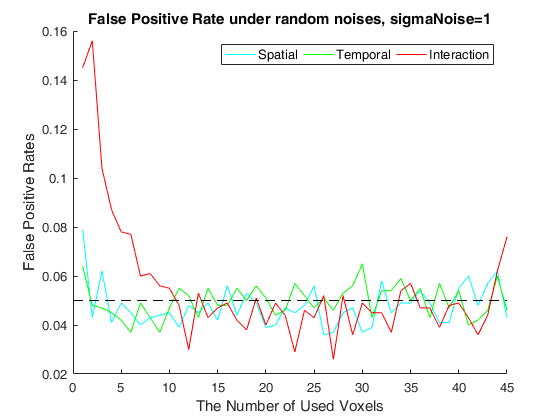
\includegraphics[scale=0.55]{0C__Users_Hao_Dropbox_NewtermPHD_TERM2_SS9833B_Analysis_of_brain_imaging_data_Report_MANOVA_Sig.png}}\subfloat{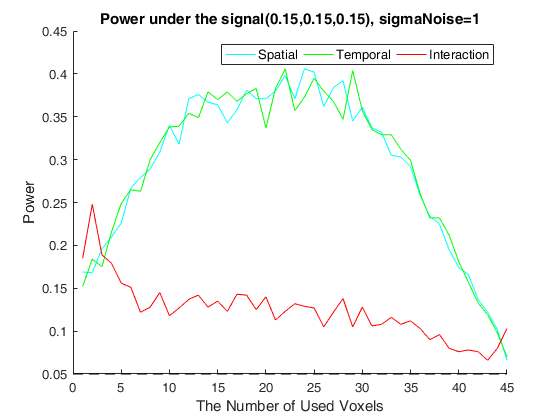
\includegraphics[scale=0.55]{1C__Users_Hao_Dropbox_NewtermPHD_TERM2_SS9833B____s_of_brain_imaging_data_Report_MANOVA_Power.png}}
\par\end{centering}

\centering{}\protect\caption{{\footnotesize{}MANOVA Using the first $N$ voxels ($N=1,\ldots,45$):
The left figure shows the false positive rates for detecting each
term from 1000 simulations of random noises. The right figure shows
the power for detecting each term from 1000 simulations of signals,
with 0.15 scale for each term. Under both cases, the variance for
the random error term is 1.}\label{fig:MANOVA1} }
\end{figure}


\begin{figure}[H]
\centering{}(0 indicates there is ).\subfloat{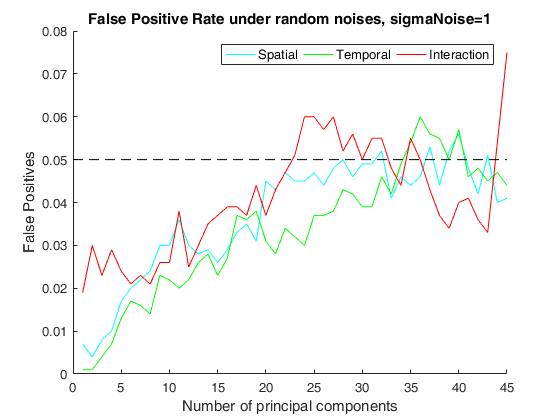
\includegraphics[scale=0.55]{2C__Users_Hao_Dropbox_NewtermPHD_TERM2_SS9833B____of_brain_imaging_data_Report_MANOVA_PCA_Sig.png}}\subfloat{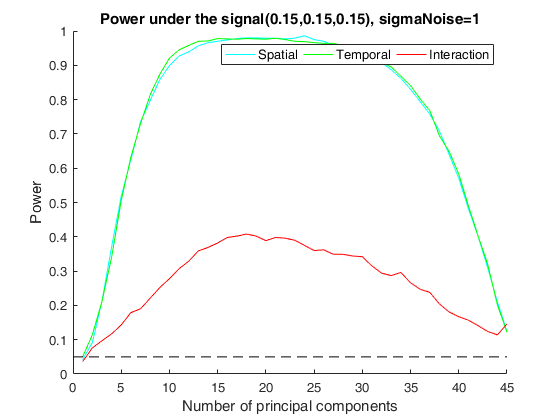
\includegraphics[scale=0.55]{3C__Users_Hao_Dropbox_NewtermPHD_TERM2_SS9833B_____brain_imaging_data_Report_MANOVA_PCA_Power.png}}\protect\caption{{\footnotesize{}CV-MANOVA using the first $N$ principal components
of voxels: The left figure shows the false positive rates for detecting
each term from 1000 simulations of random noises. The right figure
shows the power for detecting each term from 1000 simulations of signals,
with 0.15 scale for each term. Under both cases, the variance for
the random error term is 1. ($N=1,\ldots,45$) }{\small{}\label{fig:CV-MANOVA-PCA}}}
\end{figure}


\begin{figure}[H]
\centering{}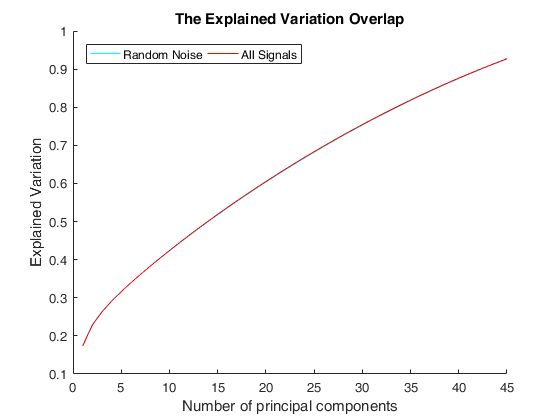
\includegraphics[scale=0.55]{4C__Users_Hao_Dropbox_NewtermPHD_TERM2_SS9833B____in_imaging_data_Report_MANOVA_PCA_Variation.png}\protect\caption{Explained Variance of PCA\label{fig:Explained-Variance-of}}
\end{figure}



\subsection{Power under Different Hypotheses}

To compare the power of different methods under different hypothese,
we did 1000 simulations under different hypothesis and the results
are shown by Figure \ref{fig:MANOVA-ss} to Figure \ref{fig:CVMANOVA-ss}.
The three digits in the legend represents if there is an effect of
the spatial pattern, the temporal pattern or the interaction, where
0 indicates no such patterns and 1 indicates the signal for the pattern
is 0.15. The curves with no markers were set to the null distribution
for performing statistical tests, because the the pattern of interest
did not exist. Hence the numbers besides the curves with markers indicate
the power for detecting the pattern in the corresponding alternative.
We can see that the CV-MANOVA enhanced the powers for both main effects
and interactions. We also found out that the CV-MANOVA was approximately
unbiased when the data is generated from random noises, but there
was a drift for the distribution of the spatial pattern when the interaction
was involved.

\begin{figure}[H]
\begin{centering}
\subfloat{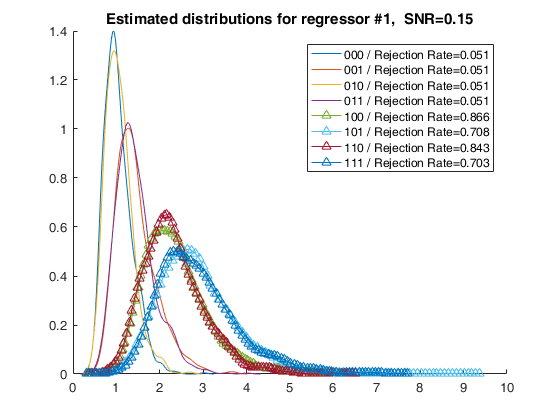
\includegraphics[scale=0.55]{5C__Users_Hao_Dropbox_NewtermPHD_TERM2_SS9833B_____imaging_data_Report_MANOVA_dist_regressor1.png}}\subfloat{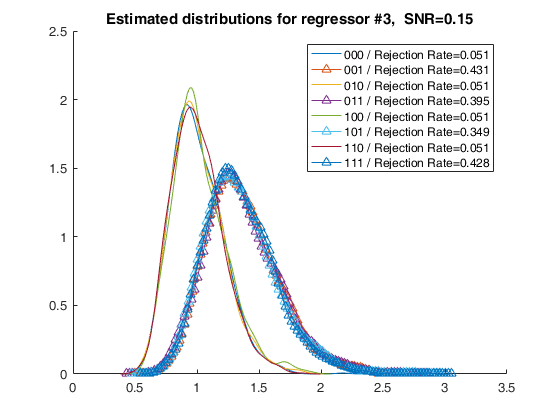
\includegraphics[scale=0.55]{6C__Users_Hao_Dropbox_NewtermPHD_TERM2_SS9833B_____imaging_data_Report_MANOVA_dist_regressor3.png}}
\par\end{centering}

\centering{}\protect\caption{MANOVA using the first $28$ principal components under difference
hypotheses: the left figure shows the power for detecting the spatial
pattern and the right figure is for the interaction.\label{fig:MANOVA-ss}}
\end{figure}


\begin{figure}[H]
\begin{centering}
\subfloat{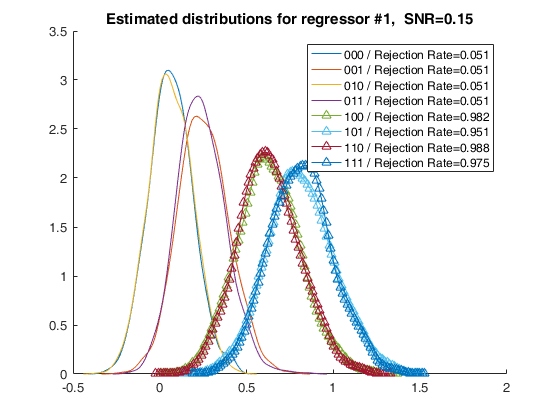
\includegraphics[scale=0.55]{9C__Users_Hao_Dropbox_NewtermPHD_TERM2_SS9833B____maging_data_Report_CVMANOVA_dist_regressor1.png}}\subfloat{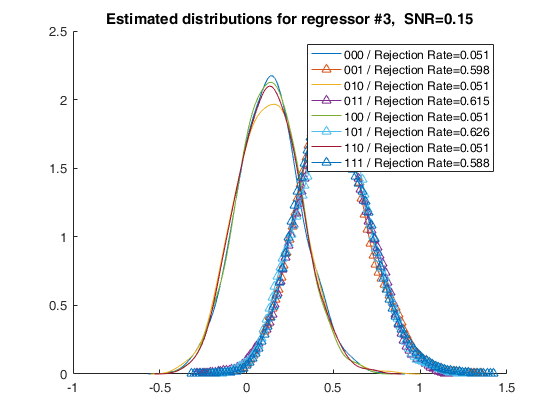
\includegraphics[scale=0.55]{10C__Users_Hao_Dropbox_NewtermPHD_TERM2_SS9833B___maging_data_Report_CVMANOVA_dist_regressor3.png}}
\par\end{centering}

\centering{}\protect\caption{CV-MANOVA under difference hypotheses: the left figure shows the power
for detecting the spatial pattern and the right figure is for the
interaction.\label{fig:CVMANOVA-ss}}
\end{figure}



\subsection{Noise Tolerance of MANOVA and CVMANOVA}

In order to see how the power of each method is related the signal-noise-ratio
(SNR), we did 1000 simulations with four different SNR's. The null
hypothesis for each method was set as random noises. Figure \ref{fig:MANOVA-SNR}
to Figure \ref{fig:CVMANOVA-SNR} show that the power of each method
increased dramatically as the SNR increased.

\begin{figure}[H]
\begin{centering}
\subfloat{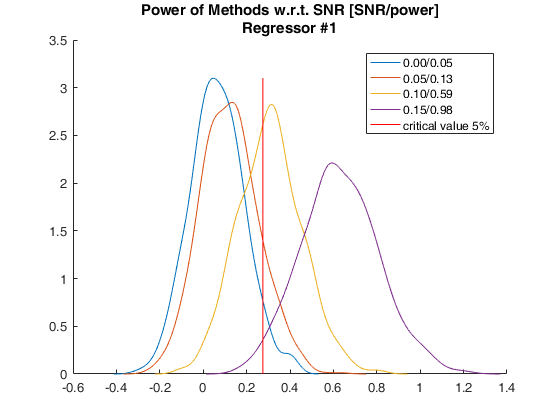
\includegraphics[scale=0.55]{7C__Users_Hao_Dropbox_NewtermPHD_TERM2_SS9833B____imaging_data_Report_MANOVA_power_regressor1.png}}\subfloat{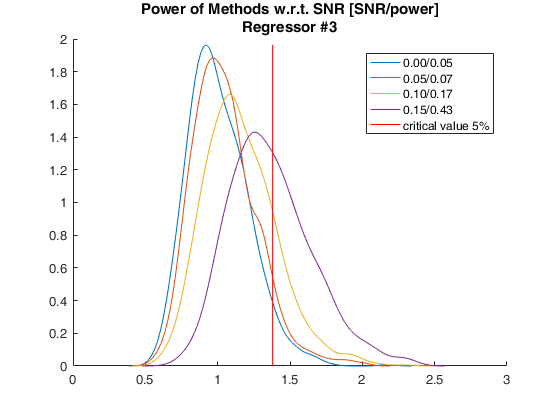
\includegraphics[scale=0.55]{8C__Users_Hao_Dropbox_NewtermPHD_TERM2_SS9833B____imaging_data_Report_MANOVA_power_regressor3.png}}
\par\end{centering}

\centering{}\protect\caption{Power v.s. SNR for MANOVA using the first $28$ principal components
under difference hypotheses.\label{fig:MANOVA-SNR}}
\end{figure}


\begin{figure}[H]
\centering{}\subfloat{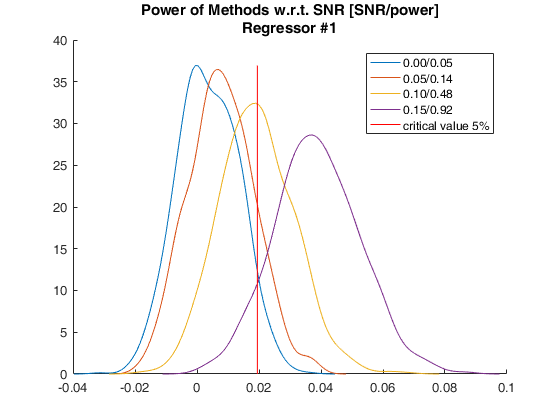
\includegraphics[scale=0.55]{11C__Users_Hao_Dropbox_NewtermPHD_TERM2_SS9833B___aging_data_Report_CVMANOVA_power_regressor1.png}}\subfloat{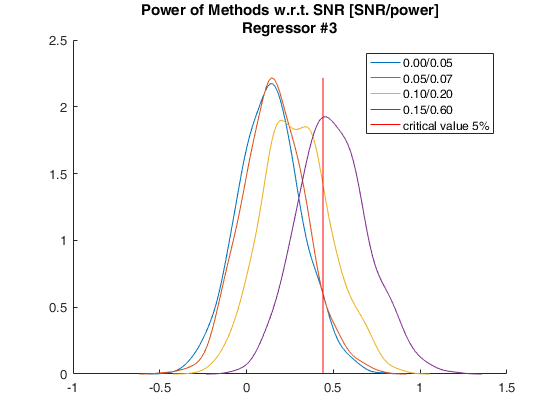
\includegraphics[scale=0.55]{12C__Users_Hao_Dropbox_NewtermPHD_TERM2_SS9833B___aging_data_Report_CVMANOVA_power_regressor3.png}}\protect\caption{Power v.s. SNR for CVMANOVA \label{fig:CVMANOVA-SNR}}
\end{figure}


\bibliographystyle{unsrt}
\phantomsection\addcontentsline{toc}{section}{\refname}\nocite{*}
\bibliography{ref}

\end{document}
